% print no page number
\thispagestyle{empty}

\chapter{Δημιουργία περιεχομένου με τη χρήση Μηχανικής Μάθησης}

Αυτό το κεφάλαιο περιγράφει την διαδικασία σχεδιασμού και υλοποίησης των μοντέλων που αναπτύχθηκαν με σκοπό την παραγωγή επιπέδων, παρόμοιων χαρακτηριστικών με τα επίπεδα που αναλύθηκαν στον κεφάλαιο 2. Η υλοποίηση είναι μια εφαρμογή Machine Learning Content Generation (MLCG). Αυτή η υλοποίηση αποτελεί μια απόδειξη, από την θεωρία στην πράξη ότι Deep Neural Networks και συγκεκριμένα GANs μπορούν να χρησιμοποιηθούν για την κατασκευή περιεχομένου.
\par
Η υλοποίηση περιλάμβανε την ολοκλήρωση πολλών επιμέρους κομματιών, κάποια από τα οποία δεν χρησιμοποιήθηκαν τελικά στην εκπαίδευση του τελικού μοντέλου. Κάτι το οποίο είναι συχνό και αναμενόμενο όταν υλοποιούνται εφαρμογές τέτοιας πολυπλοκότητας. Για παράδειγμα υλοποιήθηκαν μέθοδοι που πρόσθεταν θόρυβο στις διακριτές τιμές της εισόδου ώστε να μετατρέπονται σε συνεχείς τιμές με κανονική κατανομή. Αυτό το κομμάτι θεωρήθηκε ότι τελικά δεν προσφέρει στην απόδοση του συστήματος οπότε δεν χρησιμοποιείται στα παραδείγματα που θα αναλυθούν. Παραμένει κομμάτι της υλοποίησης χωρίς όμως να συνεισφέρει στο τελικό αποτέλεσμα.

\section{Τεχνική περιγραφή}
Το σύστημα MLCG αναπτύχθηκε στην γλώσσα\textit{Python}, μια από τις πιο διαδεδομένες γλώσσες για υλοποιήσεις Μηχανικής Μάθησης. Η έκδοση που χρησιμοποιήθηκε είναι η 3.7 και είναι ιδιαίτερα σημαντική καθώς αυτή είναι η πιο πρόσφατη έκδοση που υποστηρίζει μερικές από τις βιβλιοθήκες που χρησιμοποιήθηκαν. 
Μερικές από τις πιο σημαντικές βιβλιοθήκες και εργαλεία που χρησιμοποιήθηκαν:

\begin{description}
\item[$\bullet$ Numpy] Βιβλιοθήκη για επιστημονικές εφαρμογές και υπολογισμούς.
\item[$\bullet$ Tensorflow] Αποτελεί ένα ολοκληρωμένο σύστημα για εφαρμογές Machine Learning με υποστήριξη για πολλές γλώσσες προγραμματισμού. 
\item[$\bullet$ Keras] Αποτελεί την βιβλιοθήκη σε Python για την χρησιμοποίηση του συστήματος Tensorflow σε εφαρμογές ανεπτυγμένες σε αυτή την γλώσσα.
\end{description}


\section{Δεδομένα εκπαίδευσης}
Όπως αναλύθηκε και στο κεφάλαιο σχετικά με την υλοποίηση του PCG συστήματος σε Python, το dataset αποτελείται από αρχεία κειμένου, όπου το κάθε αρχείο αντιστοιχεί σε ένα επίπεδο. Για την εκπαίδευση του μοντέλου, δημιουργήθηκαν εκατοντάδες τέτοια αρχεία και αυτά αντιστοιχούν στο dataset μας.
\par
Όπως σε όλες τις εφαρμογές Μηχανικής Μάθησης, τα δεδομένα του dataset δεν δίνονται κατευθείαν στο μοντέλο για εκπαίδευση αλλά περνάνε από διάφορες μεθόδους προεργασίας ώστε να εξασφαλίσουμε καλύτερα και πιο αξιόπιστα αποτελέσματα.


\subsection{Χαρακτηριστικά του dataset}
Το κάθε επίπεδο είναι ένας πίνακας 900 στοιχείων, όπου το κάθε στοιχείο αντιστοιχεί σε ένα κελί στην 30x30 grid απεικόνιση του επιπέδου. Μόλις το PCG σύστημα δημιουργεί ένα επίπεδο, το μετατρέπει στην αναπαράσταση του αρχείου και το αποθηκεύει ώστε να μπορεί να διαβαστεί από το σύστημα Μηχανικής Μάθησης.
\par
Απόσπασμα από αρχείο του dataset:
\begin{verbatim}
30, 30
Tile X,Tile Y,Tile Type
0,0,1
0,1,1
0,2,1
0,3,1
0,4,1
0,5,1
\end{verbatim}
Στο παραπάνω παράδειγμα βλέπουμε τις πρώτες γραμμές από ένα αρχείο επιπέδου. Η πρώτη σειρά δηλώνει το μέγεθος του επιπέδου, κάτι το οποίο προστέθηκε για πληροφοριακούς λόγους αλλά δεν χρησιμοποιείται από το MLCG. Η δεύτερη σειρά αναγράφει το είδος των στοιχείων που αντιστοιχούν στην κάθε κολόνα αντίστοιχα.
\par

\begin{itemize}
\item Η πρώτη κολόνα, Tile X δηλώνει την x συντεταγμένη του στοιχείου μέσα στο επίπεδο.
\item Η δεύτερη κολόνα, Tile Y δηλώνει την y συντεταγμένη του στοιχείου μέσα στο επίπεδο.
\item Η τρίτη κολόνα, Tile Type, δηλώνει το είδος του στοιχείου (Corridor, Wall, Room) με ένα διακριτό ακέραιο αριθμό αντίστοιχα.
\end{itemize}

\par
H αρίθμηση των στοιχείων μέσα στο grid ξεκινάει από την κάτω αριστερή γωνία, αυτό είναι το στοιχείο με συντεταγμένες 0,0 και προχωράει πρώτα στον κάθετο άξονα (Υ) και στη συνέχεια στον οριζόντιο άξονα (Χ). Το τελευταίο στοιχείο που αναγράφετε με συντεταγμένες 29,29 αντιστοιχεί στην πάνω δεξιά γωνία του grid.

\subsection{Προ επεξεργασία Δεδομένων}
Πριν από το στάδιο της εκπαίδευσης, τα δεδομένα που θα εισάγουμε στο σύστημα πρέπει να περάσουν από το στάδιο της προ επεξεργασίας ώστε να πληρούν κάποιες προϋποθέσεις.
\par
Αρχικά γίνετε μια αλλαγή της διακριτής τιμής του κάθε στοιχείου για να τα μεταφέρουμε από το εύρος [0, 2] στο εύρος [-1, 1] το οποίο είναι το εύρος που θέλουμε να παραμείνουν οι τιμές μας και κατά την εκπαίδευση μέσα στους νευρώνες του δικτύου. Οπότε εφαρμόζουμε μια αλλαγή τιμής:
\begin{itemize}
\item Η τιμή 0 μετατρέπεται σε -1
\item Η τιμή 1 μετατρέπεται σε 0
\item Η τιμή 2 μετατρέπεται σε 1
\end{itemize}

\par
Το δεύτερο κομμάτι αφορά το είδος του μοντέλου που θέλουμε να εκπαιδεύσουμε. Στην υλοποίηση της εργασίας αναπτύχθηκαν δύο διαφορετικά μοντέλα GANs, το Dense και το Convolutional. Το κάθε μοντέλο λόγω των επιπέδων που έχει, δέχεται την είσοδο σε διαφορετική μορφή. Το Dense μοντέλο δέχεται ως είσοδο ένα διάνυσμα (900, 1). Επειδή το Dense μοντέλο ήταν το πρώτο που σχεδιάστηκε και αναπτύχθηκε, τα δεδομένα έχουν αυτή την μορφή όταν διαβάζονται από τα αρχεία του dataset. Το Convolutional μοντέλο δέχεται ως είσοδο έναν πίνακα (30, 30) διαστάσεων.
\par
Εάν η εκπαίδευση μας θα γίνει με το Convolutional μοντέλο, τα δεδομένα από διανυσματική μορφή (900, 1) μετατρέπονται σε πίνακα (30, 30) διαστάσεων.

\par
Υπάρχει η δυνατότητα προσθήκης θορύβου στα δεδομένα ώστε να έχουν μια καλύτερη κατανομή στον χώρο ανάμεσα στις διακριτές τιμές. Επειδή αυτό το στάδιο προσθέτει πολυπλοκότητα χωρίς να παρουσιάζει κάποια εμφανή διαφορά στα αποτελέσματα των μοντέλων, δεν χρησιμοποιήθηκε στις τελικές εκπαιδεύσεις. Παρόλαυτα υπάρχει η δυνατότητα να ενεργοποιηθεί οποιαδήποτε στιγμή από μια ρύθμιση στην υλοποίηση.


\section{Επεξεργασία Αποτελεσμάτων}
Η αντίθετη διαδικασία πρέπει να εκτελεστεί για τα αποτελέσματα των μοντέλων GAN. Η έξοδος του κάθε μοντέλου σε διαστάσεις είναι αντίστοιχη της εισόδου που δέχεται, συνεπώς το Dense μοντέλο παράγει διανύσματα (900, 1) και το Convolutional μοντέλο, πίνακα (30, 30).
\par
Τα αποτελέσματα του Convolutional μοντέλου πρέπει να μετατραπούν σε διάνυσμα (900, 1) για να αποθηκευτούν με την μορφή που έχει όλο το dataset.
\par
Επίσης τα αποτελέσματα των μοντέλων είναι σε συνεχείς τιμές και πρέπει να γίνει η μετατροπή τους στην κοντινότερη διακριτή τιμή από τις διαθέσιμες [-1, 0, 1] και στην συνέχεια να γίνει η αλλαγή τιμής όπως έγινε στην προ επεξεργασία:
\begin{itemize}
\item Η τιμή -1 μετατρέπεται σε 0
\item Η τιμή 0 μετατρέπεται σε 1
\item Η τιμή 1 μετατρέπεται σε 2
\end{itemize}


\subsection{Δειγματοληψία κατά την εκπαίδευση}
Για να παρακολουθούμε την πρόοδο της εκπαίδευσης ανά τακτές χρονικές περιόδους, ορίστηκε μια μεταβλητή που δηλώνει ανά πόσες εποχές, θα γίνετε δειγματοληψία από το μοντέλο. Επίσης μια δειγματοληψία γίνετε μόλις τελειώσει η εκπαίδευση για να έχουμε δείγμα από τον τελικό μοντέλο. 
\par
Σε κάθε δειγματοληψία, το μοντέλο εκτελείται με μια είσοδο εκπαίδευσης και με βάση τα βάρη που έχει εκείνη την στιγμή. Το αποτέλεσμα περνάει από την επεξεργασία που αναλύθηκε παραπάνω και αποθηκεύεται σε αρχείο με όνομα που να εκφράζει το στάδιο της εκπαίδευσης στο οποίο βρισκόταν το νευρωνικό όταν πάρθηκε αυτό το δείγμα.
\par
Για παράδειγμα το αρχείο \verb|combined_1000_09-03-2020_21-11-56FGAE.csv| είναι ένα δείγμα που δημιουργήθηκε από τον Generator σε συνεργασία με τον Discriminator (combined) στην εποχή 1000 της εκπαίδευσης. Τα υπόλοιπα στοιχεία δηλώνουν την ημερομηνία που εκτελέστηκε η συγκεκριμένη εκπαίδευση και ένα τυχαίο μοναδικό αλφαριθμητικό. 
\par
Το μοντέλο που παρήγαγε αυτό το δείγμα αναφέρετε στον φάκελο που είναι αποθηκευμένο \verb|cnn_gan-09_03_2020_21_08_34|, είναι το Convolutional μοντέλο (cnn) καθώς και η ημερομηνία και ώρα που ξεκίνησε η εκπαίδευση του συγκεκριμένου μοντέλου.

\subsection{Αποθήκευση μοντέλου}
Το κάθε μοντέλο που εκπαιδεύεται αποθηκεύεται η αρχιτεκτονική του και τα βάρη του σε ειδικά αρχεία ώστε να μπορούμε οποιαδήποτε στιγμή να τα φορτώσουμε και να τα εκτελέσουμε. Η αποθήκευση γίνετε μέσα στον φάκελο του μοντέλου, που θα δημιουργηθεί μόλις ξεκινήσει η εκπαίδευση, θα αναγράφει το είδος του μοντέλου και την ημερομηνία εκπαίδευσης.
\par
Μέσα στον φάκελο του μοντέλου θα αποθηκευτούν:
\begin{description}
\item[$\bullet$ Χαρακτηριστικά του μοντέλου] Όλη η αρχιτεκτονική του μοντέλου, δηλαδή τα επίπεδα, ο αριθμός και το είδος των παραμέτρων του κάθε επιπέδου, για τον Generator και τον Discriminator. Αυτά αποθηκεύονται μέσα στον φάκελο \texttt{model\_data} στα αρχεία  \textit{generator.json} και \textit{discriminator.json} αντίστοιχα.
\item[$\bullet$ Τα βάρη του μοντέλου] Σε αντίστοιχα αρχεία \textit{generator.h5} και \textit{discriminator.h5} αποθηκεύονται τα βάρη του κάθε δικτύου.
\item[$\bullet$ Μετρικές και αποτελέσματα] Στο αρχείο \textit{results.txt} αποθηκεύονται οι τελικές μετρήσεις και αποτελέσματα της απόδοσης του κάθε μοντέλου μαζί με διάφορες παραμέτρους που έχουμε ορίσει για την εκπαίδευση και τις τιμές τους. Με αυτό τον τρόπο μπορούμε εύκολα να συγκρίνουμε τα διάφορα μοντέλα.
\item[$\bullet$ Επίπεδα που παράχθηκαν] Στον φάκελο \textit{Results} αποθηκεύονται τα επίπεδα που δημιουργήθηκαν με την δειγματοληψία που αναφέραμε παραπάνω.
\end{description}

\section{Μοντέλο Dense GAN}

Το μοντέλο GAN που αναφέρετε ως Dense είναι το πρώτο μοντέλο GAN που αναπτύχθηκε και εκπαιδεύτηκε στα πλαίσια αυτής της εργασίας. Αναφέρετε σε διάφορα παραδείγματα υλοποιήσεων GAN \cite{firstgan3} \cite{firstgan} \cite{firstgan2} και είναι πιο εύκολο στην κατανόηση και υλοποίηση. Αναφέρετε ως μοντέλο Dense επειδή η επεξεργασία των εισόδων γίνετε στα Dense επίπεδα του δικτύου.

\subsection{Αρχιτεκτονική Generator}
Το μοντέλο του Generator δικτύου, αποτελείται από 22 επίπεδα συνολικά, από τα οποία τα πρώτα 21 μπορούν να χωριστούν σε τριάδες καθώς ακολουθούν μια κοινή αρχιτεκτονική και το τελευταίο επίπεδο δημιουργεί την έξοδο με τις διαστάσεις του επιπέδου όπως τις έχουμε ορίσει. Κάθε τριάδα επιπέδου ξεκινάει με ένα Dense επίπεδο, στην συνέχεια υπάρχει ένα LeakyReLU επίπεδο \cite{leakyrelu} και το τρίτο επίπεδο εναλλάσσετε από BatchNormalization επίπεδο σε Dropout. 

\begin{description}
\item[$\bullet$ Dense επίπεδο] Το κάθε Dense επίπεδο, πέρα από το αρχικό που λαμβάνει ως είσοδο το επίπεδο ως διάνυσμα (900, 1) στοιχείων, παίρνει ως είσοδο, την έξοδο του προηγούμενου Dropout επιπέδου. Για κάθε Dense επίπεδο ορίζουμε τον αριθμό των \textit{units} που θα έχει ως έξοδο. Για παράδειγμα για το επίπεδο εισόδου ορίζουμε:
\begin{verbatim}
Dense(units=256, input_dim=self.dungeon_dimension)
\end{verbatim}
\par
Το παραπάνω επίπεδο έχει είσοδο ένα διάνυσμα (900, 1) και ως έξοδο ένα διάνυσμα (256, 1). Το μέγεθος της εισόδου πρέπει να καθοριστεί μόνο στο αρχικό επίπεδο του δικτύου, τα υπόλοιπα γνωρίζουν τι είσοδο δέχονται με βάση την έξοδο του προηγούμενου επιπέδου.  \cite{dense}
\end{description}

\begin{description}
\item[$\bullet$ LeakyReLU] Μετά από κάθε Dense επίπεδο στην κάθε τριάδα, υπάρχει ένα επίπεδο \textit{LeakyReLU}. Αυτό το επίπεδο είναι μια παραλλαγή του επιπέδου \textit{ReLU} που αναλύσαμε με την διαφορά ότι στην περίπτωση μη ενεργοποίησης του επιπέδου από την είσοδο, η έξοδος δεν είναι μηδενική όπως στο επίπεδο της \textit{ReLU} αλλά επιστρέφει ως έξοδο μια μικρή τιμή. Η συνάρτηση ενεργοποίησης της LeakyReLU ορίζετε ως:
\par
$f(x) = alpha * x,  \;\; if \;\; x < 0$
\par
$f(x) = x,  \;\; if \;\; x >= 0$
\par
To alpha είναι μια παράμετρος που μπορεί να οριστεί σε κάθε επίπεδο LeakyReLU. Στην συγκεκριμένη υλοποίηση ορίστηκε ως εξής:
\begin{verbatim}
LeakyReLU(alpha=0.2)
\end{verbatim}
\par
O ορισμός του alpha με την τιμή 0.2 έγινε μετά από έρευνα σε αντίστοιχες υλοποιήσεις και παρατηρήσεις κατά την εκπαίδευση. \cite{firstgan} \cite{firstgan2} \cite{firstgan3} 
\end{description}

\begin{description}
\item[$\bullet$ BatchNormalization] To τελευταίο επίπεδο σε κάθε τριάδα είναι είτε το επίπεδο του BatchNormalization, ή το επίπεδο Dropout. To επίπεδο του BatchNormalization όπως αναφέρει και το όνομα κανονικοποιεί την είσοδο που δέχεται. To επίπεδο Dropout απενεργοποιεί τυχαία κάποιες από τις εξόδους μετατρέποντας τις τιμές σε 0.
\par
\begin{verbatim}
BatchNormalization(momentum=0.8)
Dropout(rate=0.3)
\end{verbatim}
\par
Η παράμετρος momentum χρησιμοποιείται με την τιμή 0.8 για να βελτιώσει την απόδοση του νευρωνικού και να αυξήσει την ταχύτητα της εκπαίδευσης \cite{firstgan}. 
\par
H παράμετρος rate δηλώνει το ποσοστό επί τις εκατό των τιμών που θα γίνουν 0 στο επίπεδο Dropout.
\end{description}

\begin{description}
\item[$\bullet$ Dense επίπεδο εξόδου] To τελευταίο επίπεδο έχει ως έξοδο το διάνυσμα του παραγομένου επιπέδου στις διαστάσεις που το έχουμε ορίσει:
\par
\begin{verbatim}
Dense(np.prod(self.dungeon_shape), activation="tanh")
\end{verbatim}
\par
Σε αντίθεση με τα υπόλοιπα επίπεδα Dense που έχουν την γραμμική συνάρτηση ως συνάρτηση ενεργοποίησης, το συγκεκριμένο επίπεδο έχει την υπερβολική εφαπτομένη για να πάρουμε έξοδο στο πεδίο τιμών [-1, 1] που είναι το πεδίο τιμών που έχουμε ορίσει για τις τιμές του επιπέδου κατά την περίοδο της εκπαίδευσης.
\end{description}

\begin{verbatim}
Dense(units=256, input_dim=self.dungeon_dimension)
LeakyReLU(alpha=0.2)
BatchNormalization(momentum=0.8)

Dense(units=512)
LeakyReLU(alpha=0.2)
Dropout(rate=0.3)

Dense(units=1024)
LeakyReLU(alpha=0.2)
BatchNormalization(momentum=0.8)

Dense(units=1024)
LeakyReLU(alpha=0.2)
Dropout(rate=0.3)

Dense(units=1024)
LeakyReLU(alpha=0.2)
BatchNormalization(momentum=0.8)

Dense(units=1024)
LeakyReLU(alpha=0.2)
Dropout(rate=0.3)

Dense(units=1024)
LeakyReLU(alpha=0.2)
BatchNormalization(momentum=0.8)

Dense(np.prod(self.dungeon_shape), activation="tanh")
\end{verbatim}


\subsection{Αρχιτεκτονική Discriminator}
Το Dense μοντέλο του Discriminator δικτύου, είναι πολύ πιο μικρό από το μοντέλο του Discriminator. Αποτελείται από μόλις 5 επίπεδα στην τελική του μορφή, έγιναν και κάποιες δοκιμές με δύο επιπλέον επίπεδα Dropout αλλά στη συνέχεια αφαιρέθηκαν. Η είσοδος του δικτύου είναι ένα επίπεδο διανυσματικής μορφής με τις διαστάσεις και τις τιμές όπως τις έχουμε αναλύσει και έχει ως έξοδο μία τιμή στο συνεχές διάστημα [0, 1].
\par
Τα επίπεδα του Discriminator όπως ορίζονται στην υλοποίηση:
\begin{verbatim}
Dense(units=512, input_dim=self.dungeon_dimension)
LeakyReLU(alpha=0.2)
Dense(units=256)
LeakyReLU(alpha=0.2)
Dense(1, input_dim=self.dungeon_dimension, activation="sigmoid")
\end{verbatim}
\par
Μπορούμε να διακρίνουμε μια παρόμοια αρχιτεκτονική με τον Generator, έχουν αρχικά ένα Dense επίπεδο και στη συνέχεια ένα επίπεδο LeakyReLU. Στον Discriminator παρόλαυτα δεν υπάρχει το επίπεδο του BatchNormalization καθώς δεν χρειάζεται να κρατήσουμε τις τιμές των εξόδων σε ένα συγκεκριμένο διάστημα.
\par
To επίπεδο της εξόδου παράγει μία τιμή με συνάρτηση ενεργοποίησης την σιγμοειδή συνάρτηση, ώστε να έχουμε το αποτέλεσμα μεταξύ 0 και 1. Όπου το 0 και τιμές κοντά στο 0 δηλώνουν ότι το επίπεδο αποτελεί παράγωγο του Generator και όχι κάποιο από τα δείγματα εκπαίδευσης και το 1 δηλώνει ότι το επίπεδο είναι από τα δείγματα εκπαίδευσης ή μοιάζει τόσο πολύ που δεν μπορεί να το ξεχωρίσει ο Discriminator.

\section{Μοντέλο CNN GAN}

Το μοντέλο GAN που αναφέρετε ως CNN είναι το δεύτερο μοντέλο GAN που αναπτύχθηκε και εκπαιδεύτηκε στα πλαίσια αυτής της εργασίας. Η σχεδίαση και ανάπτυξη του βασίστηκε στα Auxiliary Classifier GAN \cite{auxgan} τα οποία έχουν αναπτυχθεί για την παραγωγή εικόνων με συγκεκριμένο είδος περιεχομένου το οποίο ορίζετε από διακριτές κλάσεις. Ο Discriminator ενός Auxiliary Classifier GAN έχει ως στόχο να αναγνωρίσει την κλάση στην οποία ανήκει η εικόνα που παράχθηκε από τον Generator. 
\par
Αν και δεν είναι αυτός ο στόχος της εργασίας, δημιουργήσαμε το μοντέλο του CNN GAN με βάση την αρχιτεκτονική των Auxiliary Classifier GANs με μερικές αλλαγές για να ταιριάζει στον σκοπό αυτής της εργασίας. Όπως αναφέρθηκε τα αποτελέσματα του CNN GAN θεωρήθηκαν ως καλύτερης ποιότητας και πρωτοτυπίας από αυτά του  Dense GAN.

\subsection{Αρχιτεκτονική Generator}
Το μοντέλο του Generator δικτύου, αποτελείται επίσης από 22 επίπεδα συνολικά αλλά σε αυτό το μοντέλο υπάρχουν εφτά διαφορετικά είδη επιπέδων. Μπορούμε και πάλι να διακρίνουμε ομάδες επιπέδων να επαναλαμβάνονται μέσα στο δίκτυο, συγκεκριμένα την τετράδα των επιπέδων  Conv2D, LeakyReLU, BatchNormalization και Dropout, την βλέπουμε τέσσερις φορές. Επιπλέον όμως βλέπουμε και άλλα επίπεδα στην αρχή και στο τέλος του δικτύου.
\par
Τα δύο αρχικά επίπεδα, Dense και Reshape έχουν ως στόχο την αλλαγή της εισόδου στο κατάλληλο μέγεθος και διαστάσεις για τα επίπεδα 
Conv2D. Επίσης το ίδιο ισχύει και για το επίπεδο εξόδου Reshape που έχει ως στόχο να μετατρέψει την έξοδο στις διαστάσεις του επιπέδου που περιμένουμε να παραχθεί από το δίκτυο.
\par

\begin{verbatim}
Dense(units=900, input_shape=(self.latent_size,))
Reshape(target_shape=self.dungeon_shape)

Conv2D(32, 3, padding='same', strides=2)
LeakyReLU(alpha=0.2)
BatchNormalization(momentum=0.8)
Dropout(0.3)

Conv2D(64, 3, padding='same', strides=1)
LeakyReLU(alpha=0.2)
BatchNormalization(momentum=0.8)
Dropout(0.3)

Conv2D(128, 3, padding='same', strides=2)
LeakyReLU(alpha=0.2)
BatchNormalization(momentum=0.8)
Dropout(0.3)

Conv2D(256, 3, padding='same', strides=1)
LeakyReLU(alpha=0.2)
BatchNormalization(momentum=0.8)
Dropout(0.3)

Flatten()
Dense(units=900)
BatchNormalization(momentum=0.8)

Reshape(target_shape=self.dungeon_shape)
\end{verbatim}

\begin{description}
\item[$\bullet$ Reshape] To επίπεδο Reshape δεν εφαρμόζει καμία συνάρτηση στα δεδομένα αλλά αλλάζει την διάταξη τους ώστε να πάρουν άλλο σχήμα και διαστάσεις. Είναι πολύ χρήσιμο επίπεδο για περιπτώσεις όπως σε αυτή την υλοποίηση που τα δεδομένα δεν έχουν τις σωστές διαστάσεις για να δοθούν ως είσοδος σε ένα επίπεδο Conv2D.
\end{description}

\begin{description}
\item[$\bullet$ Conv2D] To επίπεδο που επεξεργάζεται τις τιμές των δεδομένων μέσα από την εφαρμογή μιας συνάρτησης συνέλιξης των δεδομένων με έναν πυρήνα συνέλιξης. \cite{conv2d}
\par
\begin{verbatim}
Conv2D(32, 3, padding='same', strides=2)
Dropout(rate=0.3)
\end{verbatim}
\par
Η πρώτη παράμετρος ορίζει τον αριθμό των διαστάσεων της εξόδου.
\par
Η δεύτερη παράμετρος ορίζει το μέγεθος του πυρήνα με τον οποίο θα γίνει η συνέλιξη, για παράδειγμα ο αριθμός 3 ορίζει έναν πυρήνα 3x3 διαστάσεων.
\par
H παράμετρος padding ορίζει εάν θα προστεθούν επιπλέον στοιχεία για να μην μειωθεί το μέγεθος των δεδομένων λόγω της συνέλιξης, με τιμή 'same' ορίζουμε ότι δεν θέλουμε να μειωθεί το μέγεθος των δεδομένων.
\par
H παράμετρος strides ορίζει πόσα "βήματα" θα κάνει κάθε φορά ο πυρήνας της συνέλιξης πάνω στα δεδομένα.
\end{description}


\subsection{Αρχιτεκτονική Discriminator}
Αντίστοιχα με το Discriminator μοντέλο του Dense δικτύου, έτσι και του CNN είναι πολύ πιο μικρό σε σχέση με τον Generator. Παρατηρούμε ομοιότητες με το μοντέλο του Generator του CNN αλλά και με το Discriminator του Dense.

\begin{verbatim}
Conv2D(32, 3, padding='same', strides=2, input_shape=self.dungeon_shape)
LeakyReLU(0.2)
Dropout(0.3)

Conv2D(64, 3, padding='same', strides=1)
LeakyReLU(0.2)
Dropout(0.3)

Flatten()
Dense(1, activation="sigmoid")

\end{verbatim}


\section{Εκπαίδευση GAN}
Για την εκπαίδευση των δύο GAN χρησιμοποιήθηκε το ίδιο dataset όπως αυτό δημιουργήθηκε από την υλοποίηση του PCG. Το dataset αποτελείται από 114 αρχεία όπου το κάθε αρχείο αντιστοιχεί σε ένα επίπεδο. Πριν ξεκινήσει η διαδικασία την εκπαίδευσης, φορτώνονται όλα τα επίπεδα στην μνήμη και περνάνε από το στάδιο της προ επεξεργασίας για να έρθουν σε μορφή που να μπορεί να επεξεργαστούν τα δύο μοντέλα GAN.
\par
Η διαδικασία της εκπαίδευσης είναι κοινή για τα δύο μοντέλα.

\subsection{Μεταβλητές εκπαίδευσης}
Κατά την δημιουργία του μοντέλου ορίζονται μεταβλητές που θα χρησιμοποιηθούν στο στάδιο της εκπαίδευσης. Όλες οι μεταβλητές έχουν προ ρυθμισμένες τιμές οι οποίες βγήκαν μέσα από δοκιμές. Μερικές από τις πιο σημαντικές είναι:

\begin{description}
\item[$\bullet$ epochs] Θετικός ακέραιος αριθμός που ορίζει τον αριθμό των εποχών που θα επαναληφθεί η εκπαίδευση. Η προτεινόμενη τιμή του για αυτή την υλοποίηση είναι 50000.
\item[$\bullet$ batch\_size] Θετικός ακέραιος αριθμός που ορίζει τον αριθμό των δειγμάτων που θα δίνονται σε κάθε εποχή για εκπαίδευση. Εάν το batch\_size είναι μικρότερο του μεγέθους του dataset, τα δείγματα που θα συμμετέχουν στην εκπαίδευση επιλέγονται τυχαία με δειγματοληψία σε κάθε εποχή και χωρίς επανατοποθέτηση. Στην περίπτωση που το batch\_size είναι μεγαλύτερο του μεγέθους του dataset, ορίζετε ως batch\_size το μέγεθος του dataset. Η προτεινόμενη τιμή του για αυτή την υλοποίηση είναι 64.
\item[$\bullet$ sample] Θετικός ακέραιος αριθμός που ορίζει το διάστημα ανάμεσα στις εποχές που λαμβάνουμε ένα δείγμα επιπέδου από το μοντέλο σε εκείνο το στάδιο της εκπαίδευσης. Αυτό ορίστηκε για να μπορούμε να παρακολουθούμε την πρόοδο του δικτύου όσο εκπαιδεύεται. Η προτεινόμενη τιμή του για αυτή την υλοποίηση είναι 1000.
\item[$\bullet$ train\_discriminator] Μία δυαδική μεταβλητή που ορίζει εάν θα πρέπει να εκπαιδεύσουμε και το δίκτυο του Discriminator. Σε περίπτωση που οριστεί να μην εκπαιδευτεί, το δίκτυο του Discriminator δεν θα πραγματοποιεί διόρθωση βαρών ανά τις εποχές της εκπαίδευσης. Παρατηρήθηκαν καλύτερα αποτελέσματα όταν εκπαιδεύαμε και το δίκτυο του Discriminator. Η προτεινόμενη τιμή του για αυτή την υλοποίηση είναι \textit{True}.
\end{description}

\subsection{Είσοδος εκπαίδευσης Generator}
Για την εκπαίδευση του Generator δίνουμε ως είσοδο στο δίκτυο, δύο πίνακες που περιέχουν ίδιο αριθμό δειγμάτων όπου το κάθε δείγμα έχει την μορφή προ επεξεργασμένου επιπέδου. Ο αριθμός των δειγμάτων ορίζετε από το batch\_size. O ένας πίνακας περιέχει δείγματα από το dataset ενώ ο άλλος πίνακας περιέχει \textit{θόρυβο}, τυχαία δημιουργημένα δείγματα που έχουν τιμές στο διάστημα που ορίσαμε για τα δείγματα των επιπέδων. 
\par
Τα στοιχεία των δύο πινάκων αντιστοιχίζονται ένα προς ένα καθώς ως στόχο το δίκτυο έχει να μετατρέψει τα δείγματα του θορύβου στα αντίστοιχα δείγματα του dataset μέσα από τις μετατροπές που θα εφαρμόσει με την εισαγωγή του θορύβου και το πέρασμα του από τα επίπεδα του δικτύου. Το τελικό αποτέλεσμα συγκρίνετε με το επιθυμητό αποτέλεσμα, το επίπεδο από το dataset, και διορθώνονται τα βάρη των επιπέδων αντίστοιχα.

\subsection{Λειτουργία Generator}
Για την λειτουργία του Generator εκτός του σταδίου της εκπαίδευσης, πρέπει να του δώσουμε ως είσοδο ένα δείγμα θορύβου για να μας δημιουργήσει ένα δείγμα επιπέδου.

\subsection{Είσοδος εκπαίδευσης Discriminator}
Για την εκπαίδευση του Discriminator δίνουμε ως είσοδο έναν πίνακα και ένα διάνυσμα. Ο πίνακας περιέχει τα δείγματα που θέλουμε να αξιολογήσει ως τεχνητά από τον Generator ή από το dataset και το διάνυσμα έχει δυαδικές τιμές που δηλώνουν την πραγματική προέλευση του κάθε δείγματος με τις τιμές 0 και 1.
\par
Για να εκπαιδευτεί ο Discriminator παίρνει ως είσοδο τα επίπεδα και ελέγχει την έξοδο του εάν ταιριάζει με την αντίστοιχη τιμή για αυτό το επίπεδο με το διάνυσμα των πραγματικών τιμών. Ομοίως διορθώνει τα βάρη του στις περιπτώσεις λάθους εάν έχουμε ενεργοποιήσει την μεταβλητή train\_discriminato.


\section{Αποτελέσματα μοντέλου CNN}

\subsection{Αποτελέσματα του Generator του CNN δικτύου, με προσθήκη θορύβου}
\begin{figure}[H]
\begin{subfigure}{.5\textwidth}
  \centering
  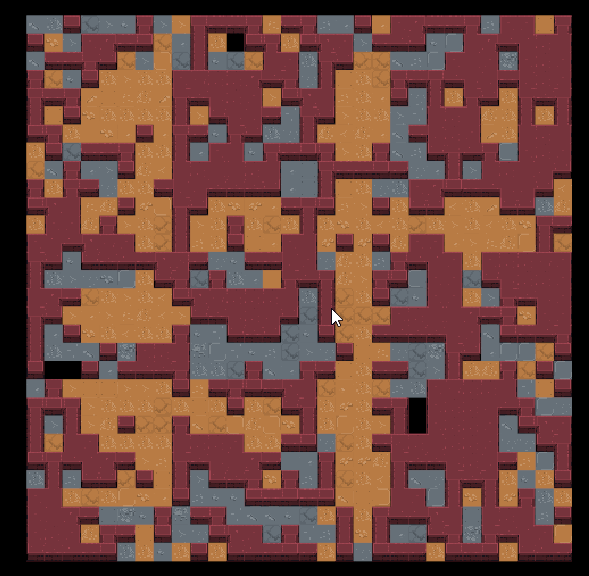
\includegraphics[width=.8\linewidth]{../images/result_images/cnn-gan-with-fuzzy/generator_1000.png}
  \caption{Επίπεδο μετά από 1000 εποχές}
  \label{fig:sfig1}
\end{subfigure}%
\begin{subfigure}{.5\textwidth}
  \centering
  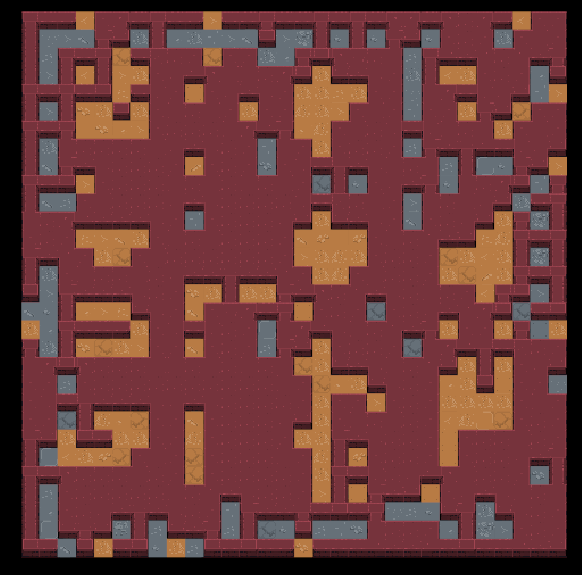
\includegraphics[width=.8\linewidth]{../images/result_images/cnn-gan-with-fuzzy/generator_3000.png}
  \caption{Επίπεδο μετά από 3000 εποχές}
  \label{fig:sfig2}
\end{subfigure}
\begin{subfigure}{.5\textwidth}
  \centering
  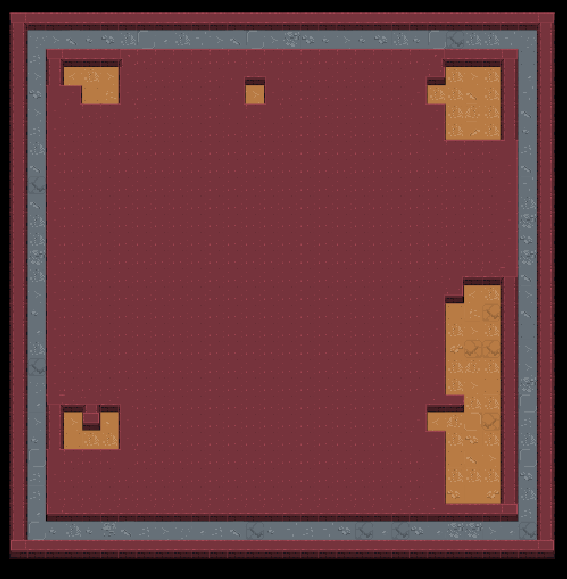
\includegraphics[width=.8\linewidth]{../images/result_images/cnn-gan-with-fuzzy/generator_7000.png}
  \caption{Επίπεδο μετά από 7000 εποχές}
  \label{fig:sfig2}
\end{subfigure}
\begin{subfigure}{.5\textwidth}
  \centering
  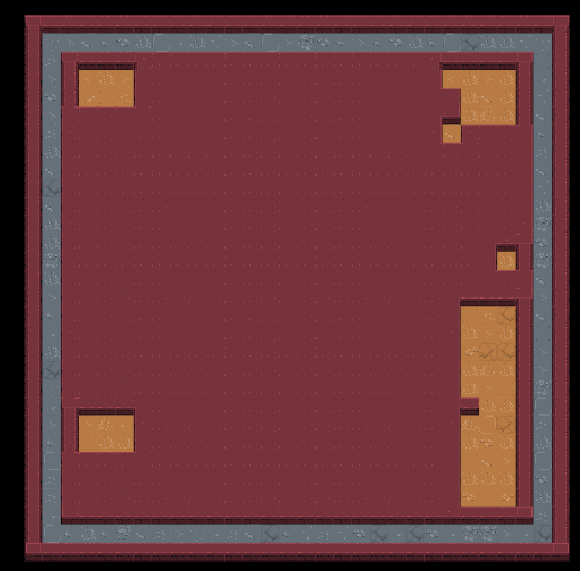
\includegraphics[width=.8\linewidth]{../images/result_images/cnn-gan-with-fuzzy/generator_10000.png}
  \caption{Επίπεδο μετά από 10000 εποχές}
  \label{fig:sfig2}
\end{subfigure}
\caption{Επίπεδα που δημιούργησε κατά την εκπαίδευση το μοντέλο του Generator χωρίς σύνδεση με το μοντέλο του Discriminator, με προσθήκη θορύβου στα δεδομένα εισόδου.}
\label{fig:fig}
\end{figure}

\subsection{Αποτελέσματα του Generator του CNN δικτύου, χωρίς προσθήκη θορύβου}
\begin{figure}[H]
\begin{subfigure}{.5\textwidth}
  \centering
  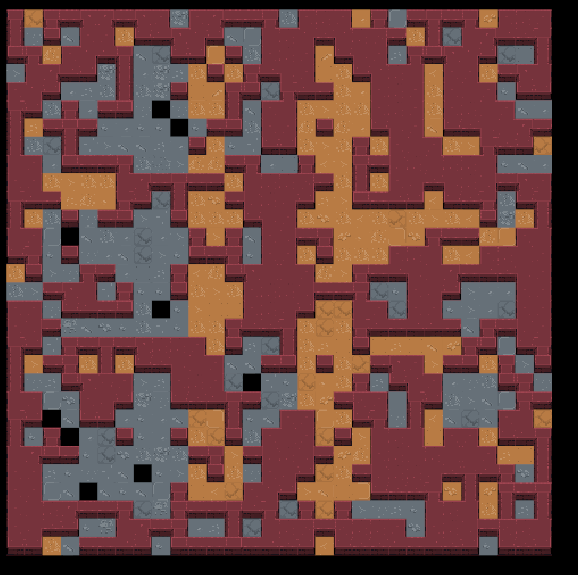
\includegraphics[width=.8\linewidth]{../images/result_images/cnn-gan/generator_1000.png}
  \caption{Επίπεδο μετά από 1000 εποχές}
  \label{fig:sfig1}
\end{subfigure}%
\begin{subfigure}{.5\textwidth}
  \centering
  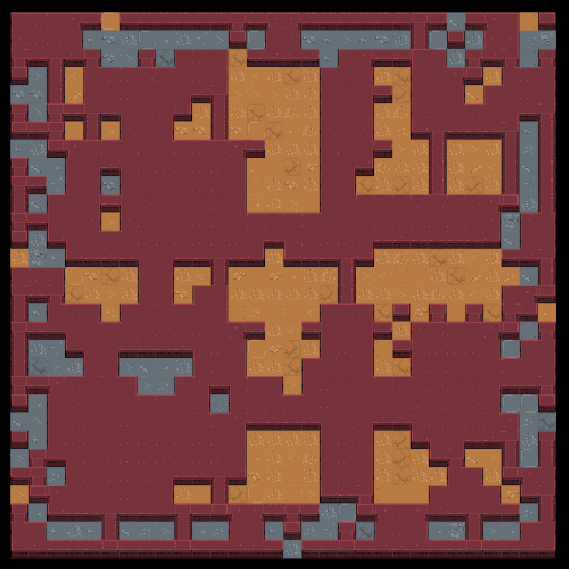
\includegraphics[width=.8\linewidth]{../images/result_images/cnn-gan/generator_3000.png}
  \caption{Επίπεδο μετά από 3000 εποχές}
  \label{fig:sfig2}
\end{subfigure}
\begin{subfigure}{.5\textwidth}
  \centering
  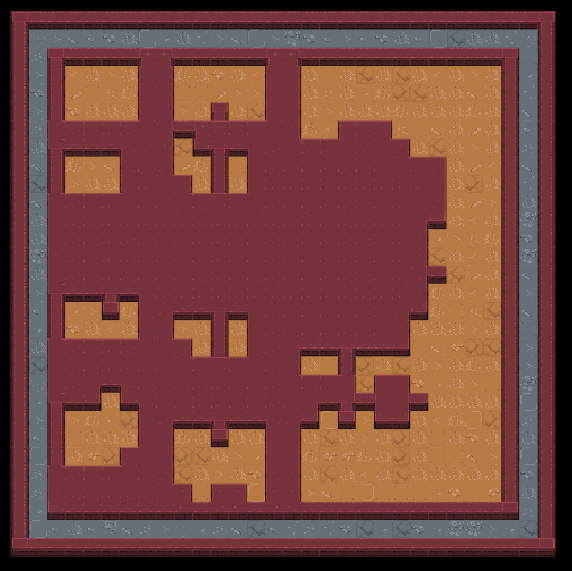
\includegraphics[width=.8\linewidth]{../images/result_images/cnn-gan/generator_7000.png}
  \caption{Επίπεδο μετά από 7000 εποχές}
  \label{fig:sfig2}
\end{subfigure}
\begin{subfigure}{.5\textwidth}
  \centering
  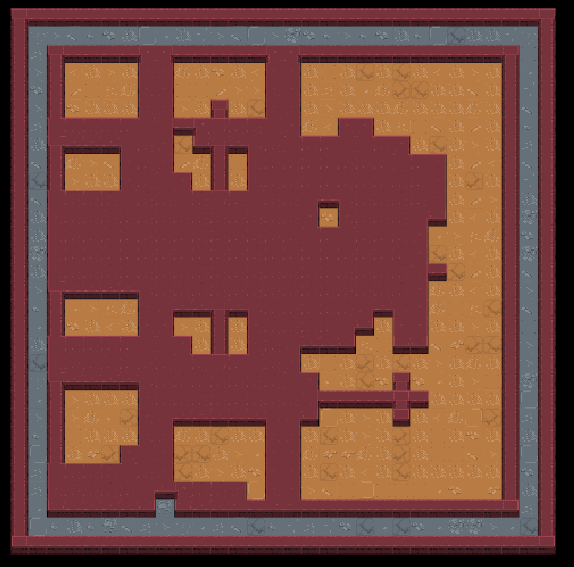
\includegraphics[width=.8\linewidth]{../images/result_images/cnn-gan/generator_10000.png}
  \caption{Επίπεδο μετά από 10000 εποχές}
  \label{fig:sfig2}
\end{subfigure}
\caption{Επίπεδα που δημιούργησε κατά την εκπαίδευση το μοντέλο του Generator χωρίς σύνδεση με το μοντέλο του Discriminator, χωρίς προσθήκη θορύβου στα δεδομένα εισόδου.}
\label{fig:fig}
\end{figure}

\subsection{Αποτελέσματα του Generator και του Discriminator του CNN δικτύου, με προσθήκη θορύβου}
\begin{figure}[H]
\begin{subfigure}{.5\textwidth}
  \centering
  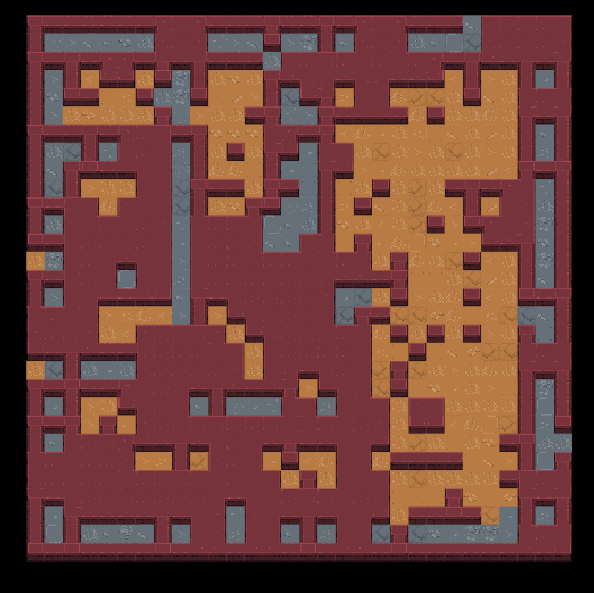
\includegraphics[width=.8\linewidth]{../images/result_images/cnn-gan-with-fuzzy/combined_1000.png}
  \caption{Επίπεδο μετά από 1000 εποχές}
  \label{fig:sfig1}
\end{subfigure}%
\begin{subfigure}{.5\textwidth}
  \centering
  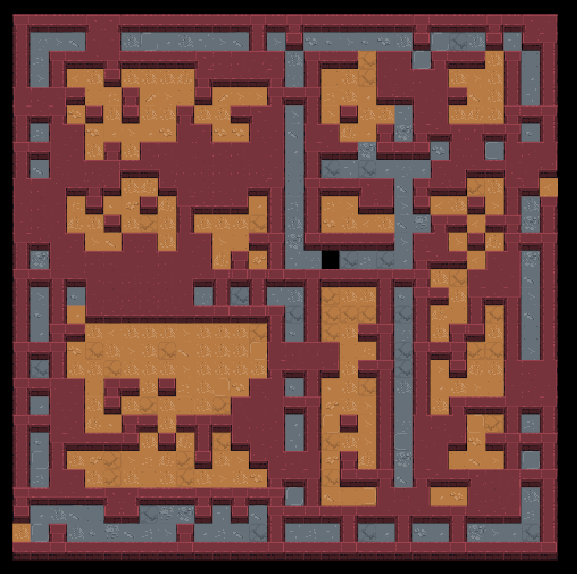
\includegraphics[width=.8\linewidth]{../images/result_images/cnn-gan-with-fuzzy/combined_3000.png}
  \caption{Επίπεδο μετά από 3000 εποχές}
  \label{fig:sfig2}
\end{subfigure}
\begin{subfigure}{.5\textwidth}
  \centering
  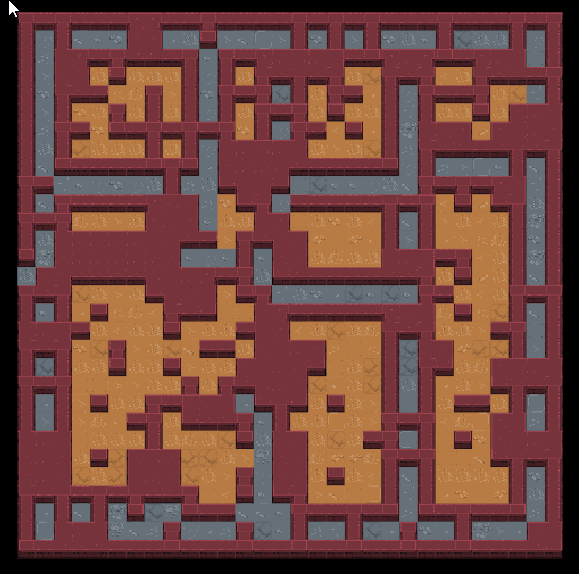
\includegraphics[width=.8\linewidth]{../images/result_images/cnn-gan-with-fuzzy/combined_7000.png}
  \caption{Επίπεδο μετά από 7000 εποχές}
  \label{fig:sfig2}
\end{subfigure}
\begin{subfigure}{.5\textwidth}
  \centering
  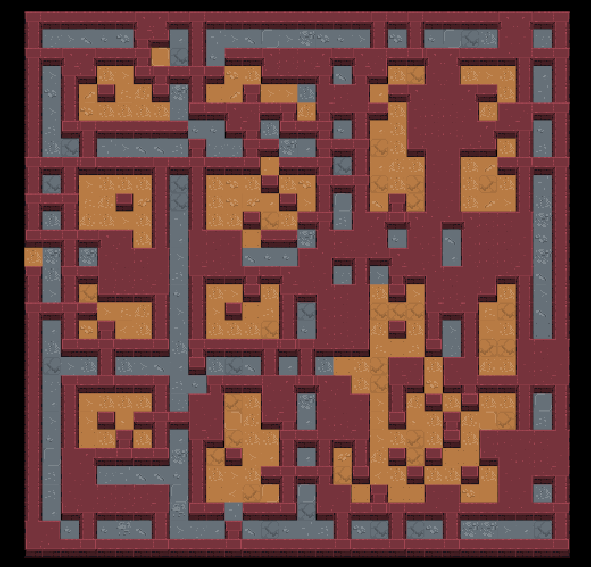
\includegraphics[width=.8\linewidth]{../images/result_images/cnn-gan-with-fuzzy/combined_10000.png}
  \caption{Επίπεδο μετά από 10000 εποχές}
  \label{fig:sfig2}
\end{subfigure}
\caption{Επίπεδα που δημιούργησε κατά την εκπαίδευση το μοντέλο του Generator με το μοντέλο του Discriminator, με προσθήκη θορύβου στα δεδομένα εισόδου.}
\label{fig:fig}
\end{figure}

\subsection{Αποτελέσματα του Generator και του Discriminator του CNN δικτύου, χωρίς προσθήκη θορύβου}
\begin{figure}[H]
\begin{subfigure}{.5\textwidth}
  \centering
  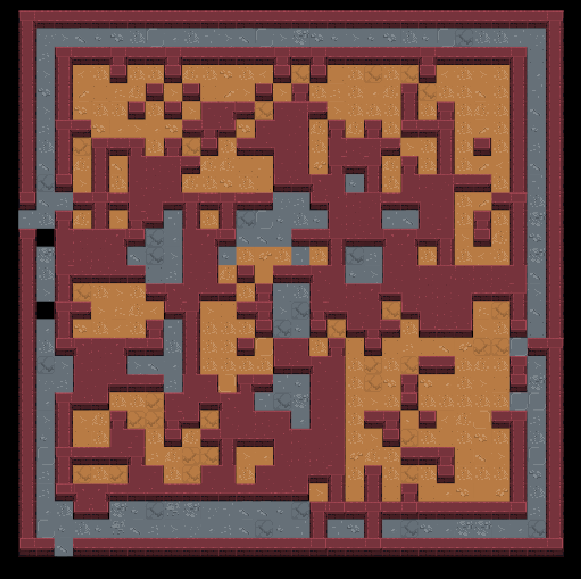
\includegraphics[width=.8\linewidth]{../images/result_images/cnn-gan/combined_1000.png}
  \caption{Επίπεδο μετά από 1000 εποχές}
  \label{fig:sfig1}
\end{subfigure}%
\begin{subfigure}{.5\textwidth}
  \centering
  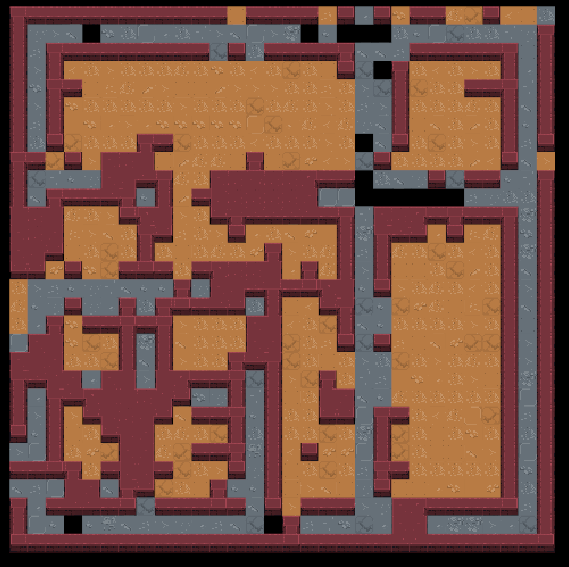
\includegraphics[width=.8\linewidth]{../images/result_images/cnn-gan/combined_3000.png}
  \caption{Επίπεδο μετά από 3000 εποχές}
  \label{fig:sfig2}
\end{subfigure}
\begin{subfigure}{.5\textwidth}
  \centering
  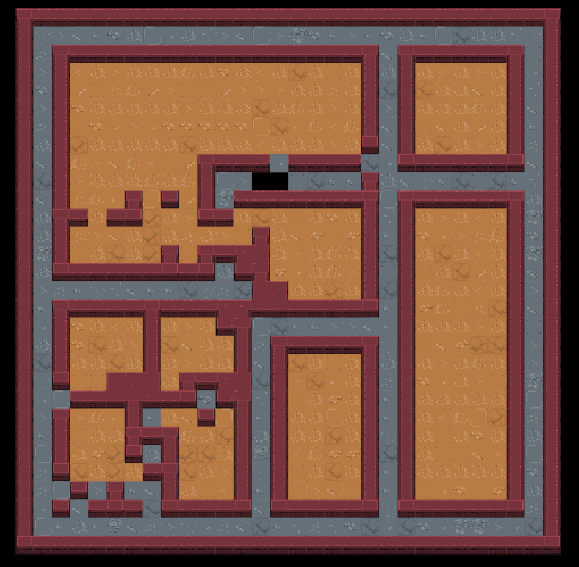
\includegraphics[width=.8\linewidth]{../images/result_images/cnn-gan/combined_7000.png}
  \caption{Επίπεδο μετά από 7000 εποχές}
  \label{fig:sfig2}
\end{subfigure}
\begin{subfigure}{.5\textwidth}
  \centering
  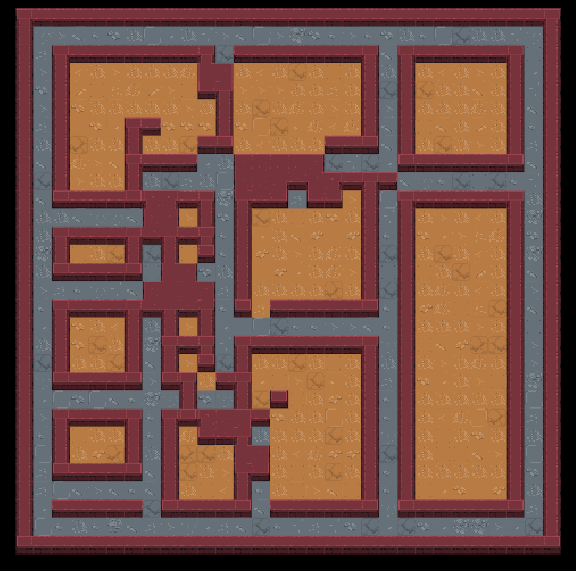
\includegraphics[width=.8\linewidth]{../images/result_images/cnn-gan/combined_10000.png}
  \caption{Επίπεδο μετά από 10000 εποχές}
  \label{fig:sfig2}
\end{subfigure}
\caption{Επίπεδα που δημιούργησε κατά την εκπαίδευση το μοντέλο του Generator με το μοντέλο του Discriminator, χωρίς προσθήκη θορύβου στα δεδομένα εισόδου.}
\label{fig:fig}
\end{figure}


\section{Αποτελέσματα μοντέλου Dense}

\subsection{Αποτελέσματα του Generator του Dense δικτύου, με προσθήκη θορύβου}
\begin{figure}[H]
\begin{subfigure}{.5\textwidth}
  \centering
  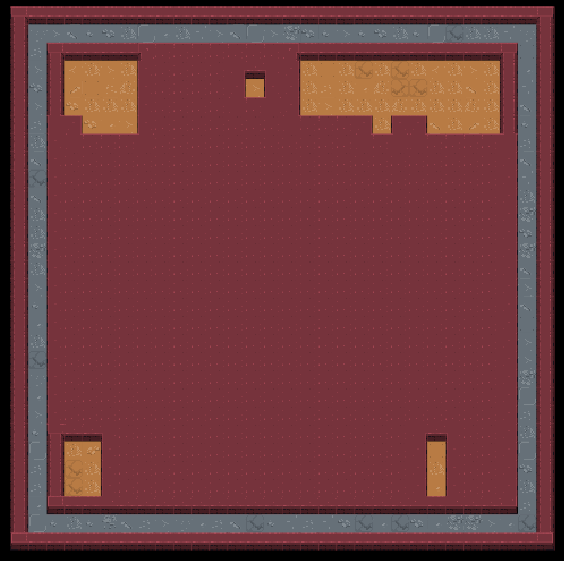
\includegraphics[width=.8\linewidth]{../images/result_images/dense-gan-with-fuzzy/generator_1000.png}
  \caption{Επίπεδο μετά από 1000 εποχές}
  \label{fig:sfig1}
\end{subfigure}%
\begin{subfigure}{.5\textwidth}
  \centering
  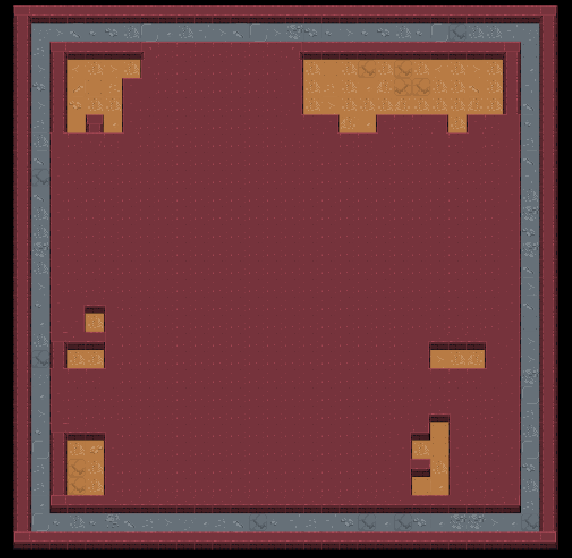
\includegraphics[width=.8\linewidth]{../images/result_images/dense-gan-with-fuzzy/generator_3000.png}
  \caption{Επίπεδο μετά από 3000 εποχές}
  \label{fig:sfig2}
\end{subfigure}
\begin{subfigure}{.5\textwidth}
  \centering
  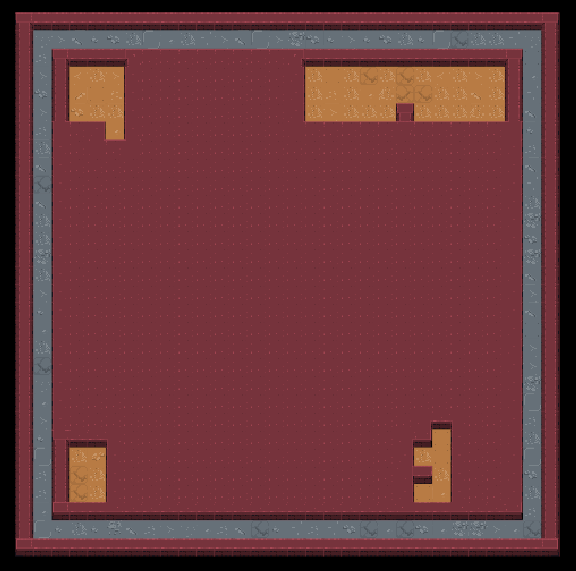
\includegraphics[width=.8\linewidth]{../images/result_images/dense-gan-with-fuzzy/generator_7000.png}
  \caption{Επίπεδο μετά από 7000 εποχές}
  \label{fig:sfig2}
\end{subfigure}
\begin{subfigure}{.5\textwidth}
  \centering
  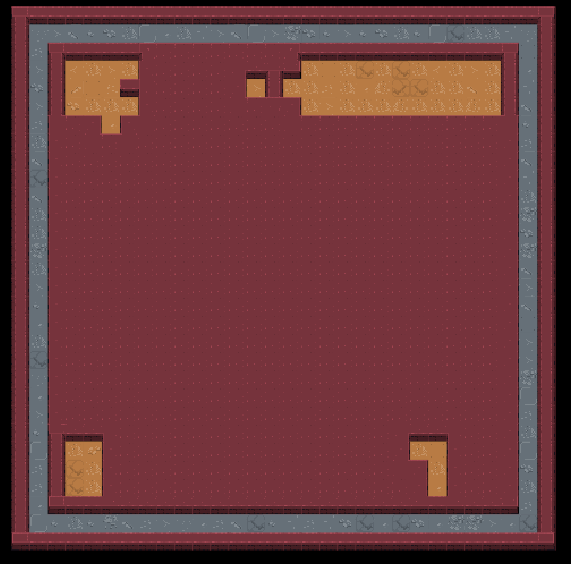
\includegraphics[width=.8\linewidth]{../images/result_images/dense-gan-with-fuzzy/generator_10000.png}
  \caption{Επίπεδο μετά από 10000 εποχές}
  \label{fig:sfig2}
\end{subfigure}
\caption{Επίπεδα που δημιούργησε κατά την εκπαίδευση το μοντέλο του Generator χωρίς σύνδεση με το μοντέλο του Discriminator, με προσθήκη θορύβου στα δεδομένα εισόδου.}
\label{fig:fig}
\end{figure}

\subsection{Αποτελέσματα του Generator του Dense δικτύου, χωρίς προσθήκη θορύβου}
\begin{figure}[H]
\begin{subfigure}{.5\textwidth}
  \centering
  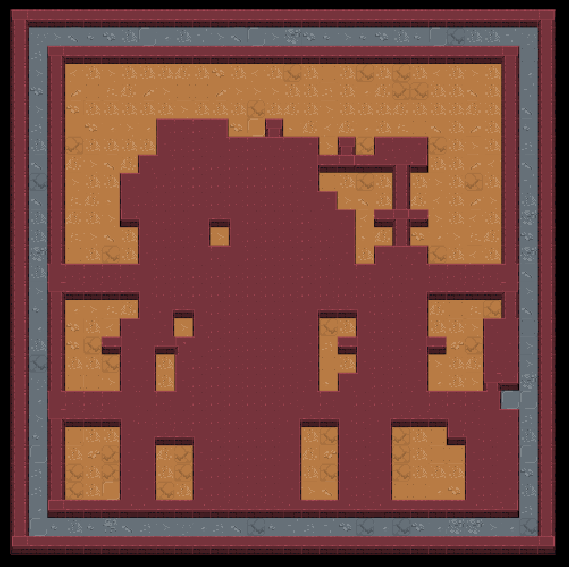
\includegraphics[width=.8\linewidth]{../images/result_images/dense-gan/generator_1000.png}
  \caption{Επίπεδο μετά από 1000 εποχές}
  \label{fig:sfig1}
\end{subfigure}%
\begin{subfigure}{.5\textwidth}
  \centering
  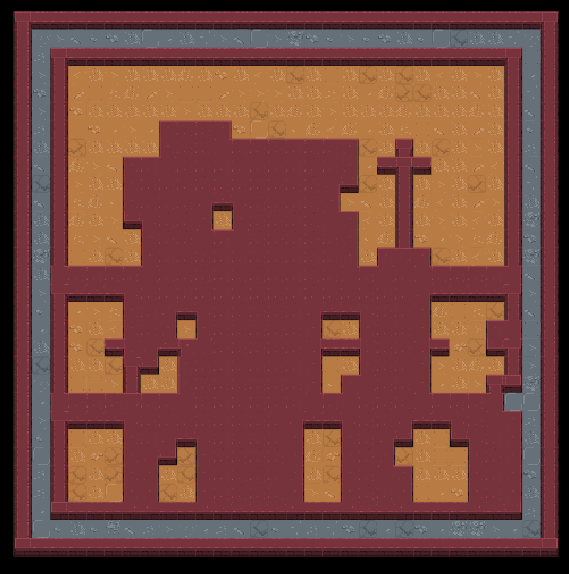
\includegraphics[width=.8\linewidth]{../images/result_images/dense-gan/generator_3000.png}
  \caption{Επίπεδο μετά από 3000 εποχές}
  \label{fig:sfig2}
\end{subfigure}
\begin{subfigure}{.5\textwidth}
  \centering
  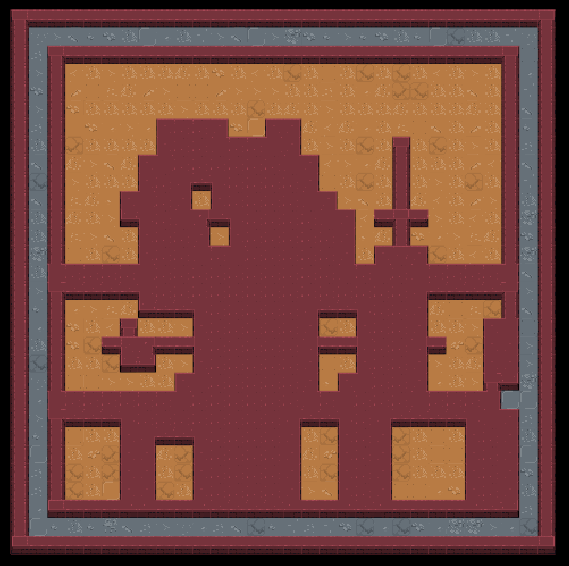
\includegraphics[width=.8\linewidth]{../images/result_images/dense-gan/generator_7000.png}
  \caption{Επίπεδο μετά από 7000 εποχές}
  \label{fig:sfig2}
\end{subfigure}
\begin{subfigure}{.5\textwidth}
  \centering
  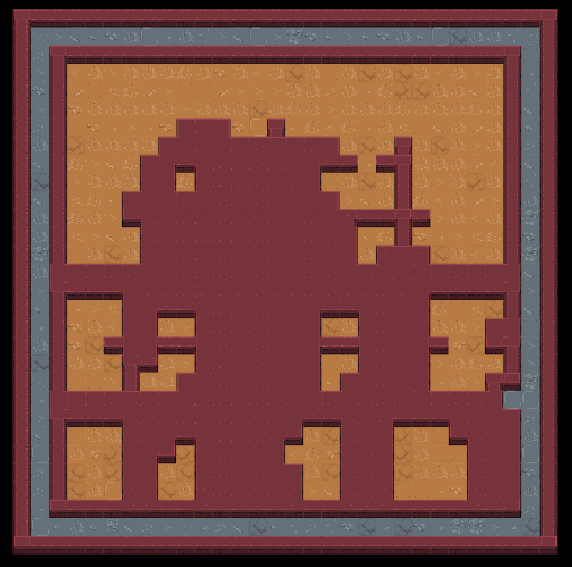
\includegraphics[width=.8\linewidth]{../images/result_images/dense-gan/generator_10000.png}
  \caption{Επίπεδο μετά από 10000 εποχές}
  \label{fig:sfig2}
\end{subfigure}
\caption{Επίπεδα που δημιούργησε κατά την εκπαίδευση το μοντέλο του Generator χωρίς σύνδεση με το μοντέλο του Discriminator, χωρίς προσθήκη θορύβου στα δεδομένα εισόδου.}
\label{fig:fig}
\end{figure}

\subsection{Αποτελέσματα του Generator και του Discriminator του Dense δικτύου, με προσθήκη θορύβου}
\begin{figure}[H]
\begin{subfigure}{.5\textwidth}
  \centering
  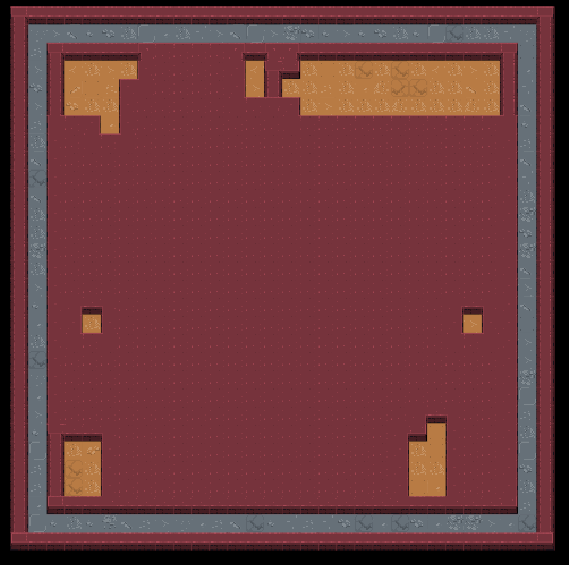
\includegraphics[width=.8\linewidth]{../images/result_images/dense-gan-with-fuzzy/combined_1000.png}
  \caption{Επίπεδο μετά από 1000 εποχές}
  \label{fig:sfig1}
\end{subfigure}%
\begin{subfigure}{.5\textwidth}
  \centering
  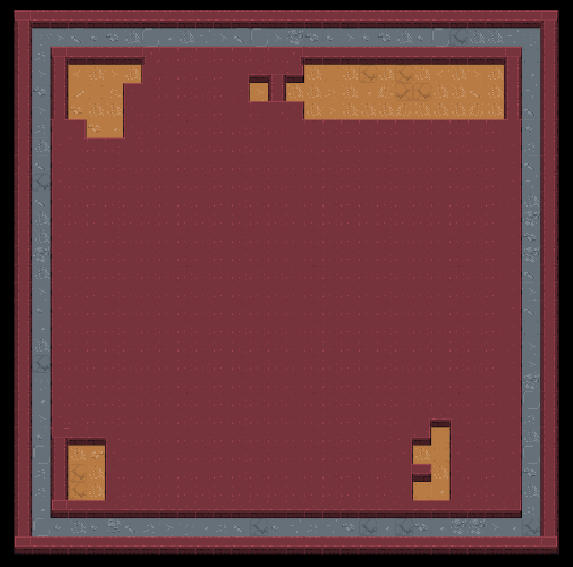
\includegraphics[width=.8\linewidth]{../images/result_images/dense-gan-with-fuzzy/combined_3000.png}
  \caption{Επίπεδο μετά από 3000 εποχές}
  \label{fig:sfig2}
\end{subfigure}
\begin{subfigure}{.5\textwidth}
  \centering
  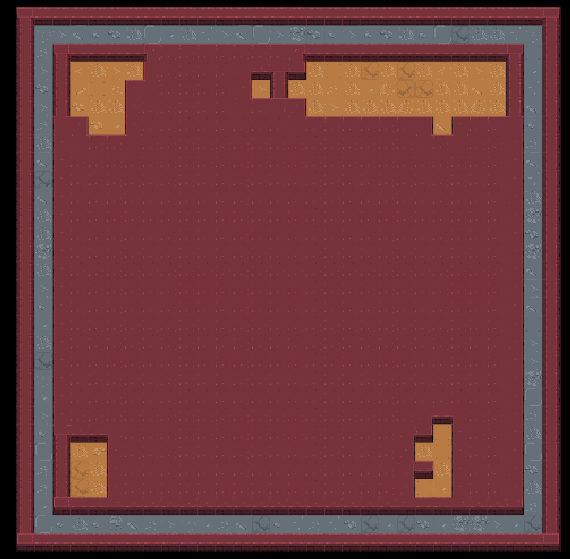
\includegraphics[width=.8\linewidth]{../images/result_images/dense-gan-with-fuzzy/combined_7000.png}
  \caption{Επίπεδο μετά από 7000 εποχές}
  \label{fig:sfig2}
\end{subfigure}
\begin{subfigure}{.5\textwidth}
  \centering
  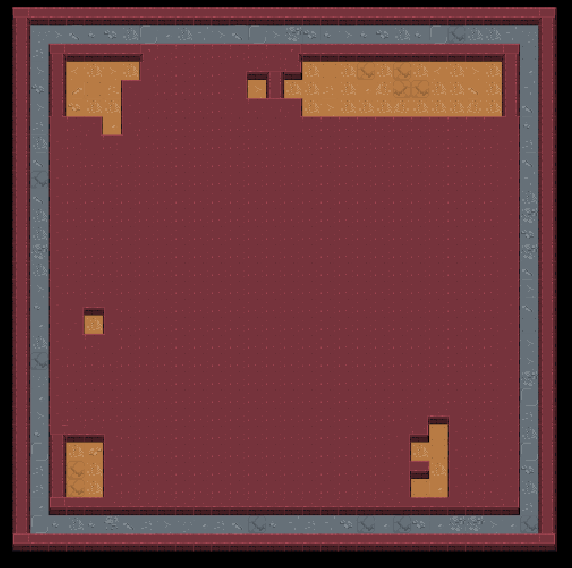
\includegraphics[width=.8\linewidth]{../images/result_images/dense-gan-with-fuzzy/combined_10000.png}
  \caption{Επίπεδο μετά από 10000 εποχές}
  \label{fig:sfig2}
\end{subfigure}
\caption{Επίπεδα που δημιούργησε κατά την εκπαίδευση το μοντέλο του Generator με το μοντέλο του Discriminator, με προσθήκη θορύβου στα δεδομένα εισόδου.}
\label{fig:fig}
\end{figure}

\subsection{Αποτελέσματα του Generator και του Discriminator του Dense δικτύου, χωρίς προσθήκη θορύβου}
\begin{figure}[H]
\begin{subfigure}{.5\textwidth}
  \centering
  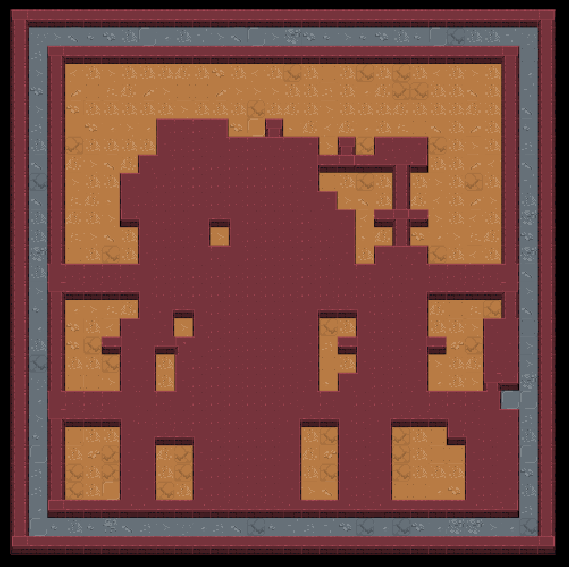
\includegraphics[width=.8\linewidth]{../images/result_images/dense-gan/generator_1000.png}
  \caption{Επίπεδο μετά από 1000 εποχές}
  \label{fig:sfig1}
\end{subfigure}%
\begin{subfigure}{.5\textwidth}
  \centering
  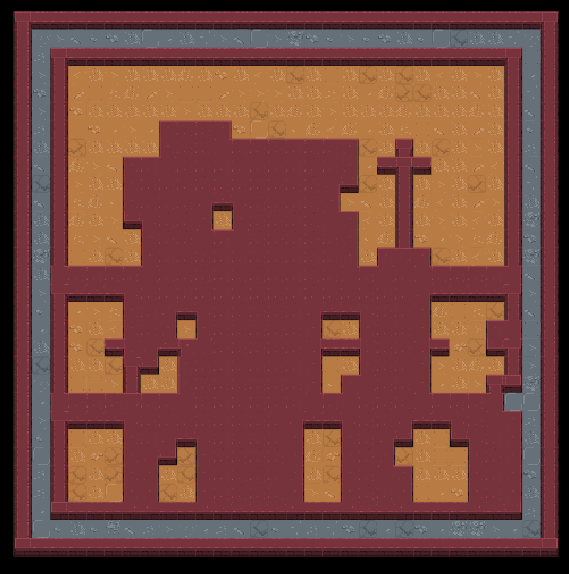
\includegraphics[width=.8\linewidth]{../images/result_images/dense-gan/generator_3000.png}
  \caption{Επίπεδο μετά από 3000 εποχές}
  \label{fig:sfig2}
\end{subfigure}
\begin{subfigure}{.5\textwidth}
  \centering
  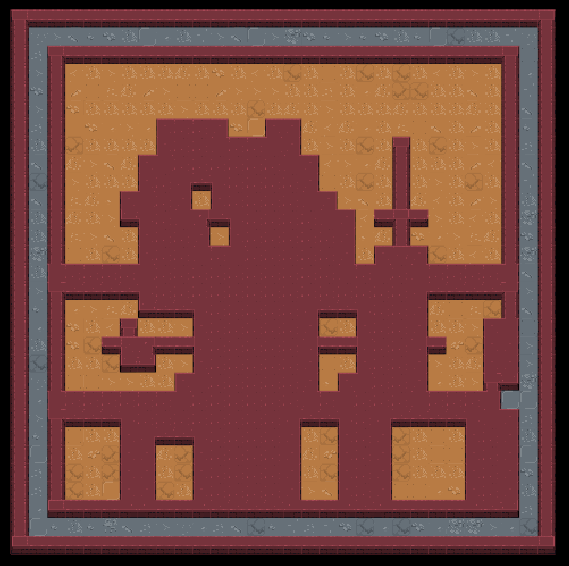
\includegraphics[width=.8\linewidth]{../images/result_images/dense-gan/generator_7000.png}
  \caption{Επίπεδο μετά από 7000 εποχές}
  \label{fig:sfig2}
\end{subfigure}
\begin{subfigure}{.5\textwidth}
  \centering
  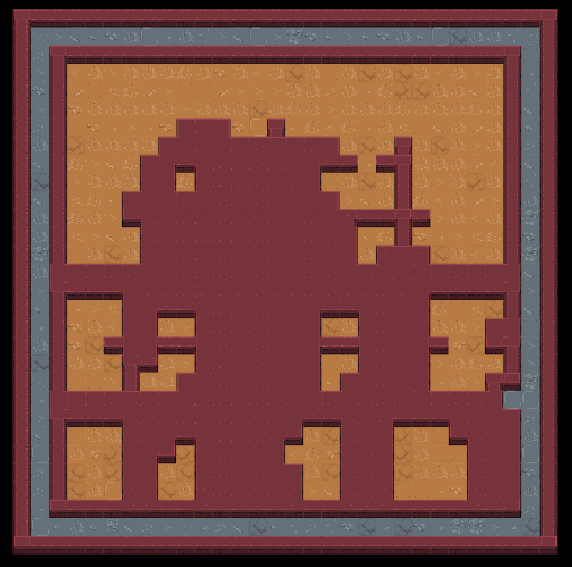
\includegraphics[width=.8\linewidth]{../images/result_images/dense-gan/generator_10000.png}
  \caption{Επίπεδο μετά από 10000 εποχές}
  \label{fig:sfig2}
\end{subfigure}
\caption{Επίπεδα που δημιούργησε κατά την εκπαίδευση το μοντέλο του Generator χωρίς σύνδεση με το μοντέλο του Discriminator, χωρίς προσθήκη θορύβου στα δεδομένα εισόδου.}
\label{fig:fig}
\end{figure}

